\documentclass[12pt , a4paper]{article}

\usepackage[french]{babel}
\usepackage [utf8] {inputenc} % utf-8 / latin1
\usepackage[T1]{fontenc}
\usepackage{aeguill} %impression de qualite des listings
\usepackage {amsmath}
\usepackage {mathpazo}
\usepackage {hyperref} %lien dynamique
\usepackage {graphicx}%image
\usepackage {fancyhdr}%entete et pied de page
\usepackage {float} %image
\usepackage {color}
\usepackage{lastpage}
\usepackage[top=2cm, bottom=2cm, left=2cm , right=2cm]{geometry}
\usepackage{vmargin}
\usepackage{listings}
\usepackage{lscape}


\definecolor{hellgelb}{rgb}{1,1,0.8}
\definecolor{colKeys}{rgb}{0,0,1}
\definecolor{colIdentifier}{rgb}{0,0,0}
\definecolor{colComments}{rgb}{0,0.5,0}
\definecolor{colString}{rgb}{0.62,0.12,0.94}

\newcommand {\TitreCours}{C++}
\newcommand {\Epoque}{GM4 - 2ème semestre}
\newcommand {\Prof}{M. Kotowicz}
\newcommand {\Auteur}{Pauline Réquéna \and Guillaume Dubuisson Duplessis \and Arnaud Faure}

\newcommand{\J}{
  \lstset{
    language=java,
    float=hbp,
    basicstyle=\ttfamily\small,
    identifierstyle=\color{colIdentifier},
    keywordstyle=\bf \color{colKeys},
    stringstyle=\color{colString},
    commentstyle=\color{colComments},
    columns=flexible,
    tabsize=5,
    frame=single,
    % frame=shadowbox,
    rulesepcolor=\color[gray]{0.5},
    extendedchars=true,
    showspaces=false,
    showstringspaces=false,
    numbers=left,
    stepnumber=5,
    firstnumber=1,
    numberstyle=\tiny,
    breaklines=true,
    % backgroundcolor=\color{hellgelb},
    captionpos=b,%
  }
}


\title{C++\\
  \vspace{0.6cm}
  \normalsize{Résolution du monde des cubes par éco-résolution} 
  \begin{center}
    % \includegraphics[scale=3.5]{./images/piton3d.jpg}
  \end{center}
}
\author{\Auteur}
\date{\today}

% UNE METHODE DE DEFINITION D'ENTETE
% \pagestyle{fancy}
% \fancyhf{}%detruit les entetes deja presents
% \renewcommand{\headrulewidth}{0.4pt}
% \renewcommand{\footrulewidth}{0.4pt}
% \lhead{\Auteur}
% \rhead{\today}
% \rfoot{\thepage\ sur \pageref{LastPage}}

% MEMO
% \lhead{haut gauche}
% \chead{centre haut}
% \rhead{haut droit}
% \lfoot{bas gauche}

% UNE AUTRE METHODE
% \pagestyle{headings}
\setmarginsrb{2.5cm}{1cm}{1cm}{1.5cm}{.5cm}{.5cm}{.5cm}{.5cm}
% \renewcommand{\sectionmark}[1]{\markright{\textsc{\TitreCours:} \thesection. \#1 \hrulefill\ \textup{page }}}
% FONCTIONNEMENT DE \setmarginsrb
% \setmarginsrb{1}{2}{3}{4}{5}{6}{7}{8}
% 1 est la marge gauche
% 2 est la marge en haut
% 3 est la marge droite
% 4 est la marge en bas
% 5 fixe la hauteur de l'entête
% 6 fixe la distance entre l'entête et le texte
% 7 fixe la hauteur du pied de page
% 8 fixe la distance entre le texte et le pied de page

% UNE DERNIERE METHODE
\pagestyle{fancy}
\fancyhf{}%supprime les entetes et pieds de page utilise par defaut par LaTeX
% \rightmark : contient le nom de la section courante
% \markright : contient le nom de la section courante
% \renewcommand{\sectionmark}[1]{\markright{\#1}}
% \renewcommand{\chaptermark}[1]{\markboth{\bsc{\chaptername~\thechapter{} :} #1}{}}
\renewcommand{\sectionmark}[1]{\markright{\thesection{} #1}}
\lhead[\thepage]{\TitreCours\ - \rightmark} 
\rhead{\Epoque}
\rfoot{\thepage\ / \pageref{LastPage}}

\fancypagestyle{plain}{ 
  \fancyhead{} 
  \renewcommand{\headrulewidth}{0pt}
}

\begin{document}
\maketitle
\thispagestyle{empty}
% \setcounter{page}{0}
\newpage
\thispagestyle{plain}% page sans entete 

\tableofcontents
\newpage
\section{Introduction}
\noindent blabla

\newpage

\section{Analyse des besoins}
\subsection{Préliminaires}
\subsubsection{Principe de l'eco-resolution}
\noindent L'éco-résolution est utilisée pour la résolution des problèmes en Intelligence Artificielle.\\
Elle se compose de 2 parties :
\begin{itemize}
\item Un protocole suivi par l’ensemble des agents, qui est un noyau indépendant du problème à résoudre
\item Un code de comportements des éco-agents spécifiques au problème à résoudre\\
\end{itemize}

\noindent Les éco-agents sont  les entités qui constituent le système.  Leur particularité est d'être en  quête perpétuelle d'un état de satisfaction.  Les éco-agents peuvent se gêner mutuellement ce qui donne
naissance à deux comportements : l'aggression des gêneurs et la fuite de ceux-ci. Ils sont également caractérisés par :
\begin{itemize}
\item Un but : il s'agit d’un autre éco-agent avec lequel il dit être en relation de satisfaction
\item Un état interne : satisfait, en recherche de satisfaction, en fuite ou en recherche de fuite
\item Des actions élémentaires : elles dépendent du domaine et correspondent aux comportements de satisfaction ou de fuite
\item La perception des gêneurs : Il s'agit de la perception des éco-agents qui empêchent l'éco-agent courant d'être satisfait ou de fuir
\item Des dépendances : les éco-agents dont l'éco-agent courant est le but. Elles sont satisfaites uniquement si cet éco-agent est satisfait. \\
\end{itemize}

\noindent Un éco-agent a la volonté d'être satisfait. Il cherche à se trouver dans un état de satisfaction. S'il est empêché par des gêneurs alors il les agresse.\\
Un éco-agent a l'obligation de fuir. Si un éco-agent est agressé, il doit trouver une place ou fuir.
Enfin un éco-agent peut effectuer 3 opérations :
\begin{itemize}
\item Agresser
\item FaireSatisfaction
\item FaireFuite
\end{itemize}


\subsubsection{Le monde des cubes}
Le monde des cubes consiste en le problème suivant : des cubes sont disposés sur une table formant des piles et l'objectif de pouvoir bouger les cubes suivant des contraintes (poser le cube A sur le cube H par exemple).\\
\noindent Prenons l'exemple de la situation suivante :
\begin{center}
	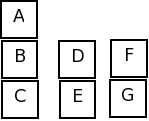
\includegraphics[scale=0.7]{../Image/1.png}
\end{center}
L'objectif est de déplacer le cube C et de le mettre sur le cube D. Cette opération sera réalisé selon les étapes suivantes :
\begin{center}
	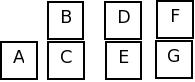
\includegraphics[scale=0.7]{../Image/2.png}
\end{center}
Le cube A est posé sur la table.
\begin{center}
	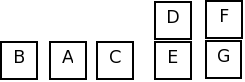
\includegraphics[scale=0.7]{../Image/3.png}	
\end{center}
Le cube B est posé sur la table, ainsi le cube C est libre.
\begin{center}
	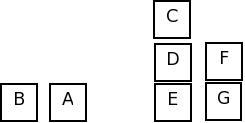
\includegraphics[scale=0.7]{../Image/4.png}	
\end{center}
Finalement, le cube C est déplacé sur le cube D.\\
Plusieurs options existent pour la résolution de ce problème : l'utilisation de robots qui déplaceraient les cubes et l'éco-résolution avec les cubes et la table comme éco-agents. Nous avons choisi cette dernière option même si de premier abord elle paraît être moins instinctive car nous pensons que ce problème illustre parfaitement l'utilisation de l'éco-résolution.
\subsection{Composition du système}
L'objectif affiché est donc de résoudre le problème du déplacement des cubes par l'éco-résolution. Tout problème possède néanmoins une base commune : la plateforme d'éco-résolution qui permet l'exécution des éco-agents et les éco-agents eux-même. 
\subsubsection{Plateforme d'éco-resolution}
\noindent La plateforme d'éco-résolution qui permet :
\begin{itemize}
\item l'ajout d'éco-agent
\item la suppression d'éco-agent
\item l'exécution des éco-agents
\end{itemize}
\subsubsection{Les éco-agents}
\noindent Les éco-agents précédemment décrits qui sont capables de réaliser principalement trois opérations :
\begin{itemize}
\item Agresser
\item FaireSatisfaction
\item FaireFuite
\end{itemize}
Les états successifs des éco-agents peuvent être décrits par l'automate suivant :
INSERTION DIAGRAMME D'ETATS/TRANSITIONS
\subsection{Les grandes fonctionnalités}
On peut distinguer les grandes fonctionnalités suivantes :
\begin{itemize}
\item créer une situation initiale : positionnement intial des cubes sur la table
\item déterminer la situation finale : positionnement final des cubes sur la table
\item démarrer la résolution
\item trace de la résolution (affichage graphique, log, etc.)
\end{itemize}

\subsection{Les étapes pour démarrer la résolution}
Nous allons maintenant résumer les différentes étapes nécessaires pour réaliser la résolution :
\begin{enumerate}
\item Création de l'éco-agent table
\item Création des  éco-agents cubes
\item Donner aux éco-agents des conditions de satisfactions ainsi que les relations de dépendance qui en découlent
\item Démarrer la résolution
\end{enumerate}


\newpage	
\section{Conclusion}
blabla
\end{document}
